\section{Introduction}
\label{sec:intro}

\begin{figure*}[t]
\centering
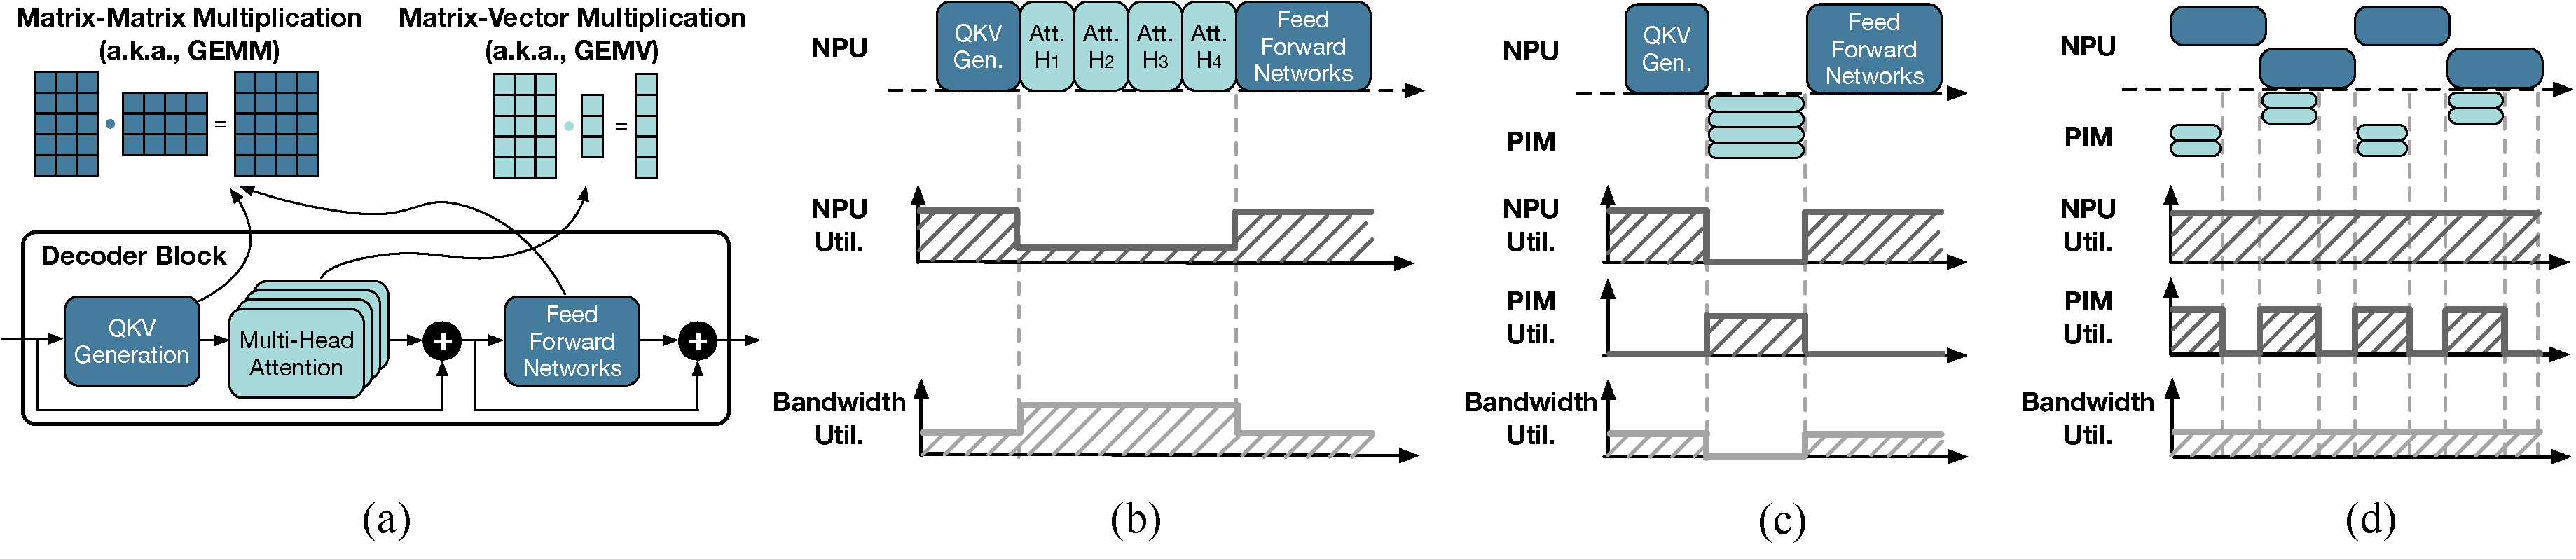
\includegraphics[width=0.95\textwidth]{figure/fig1-intro-overview.pdf}
\vspace{-3ex}
\caption{(a) Mathematical components of decoder blocks that constitute LLMs, (b) NPU-only baseline accelerator equipped with \emph{non}-PIM memory (e.g., GPU), (c) NPU+PIM integrated baseline accelerator, and (d) the proposed \neupims accelerator.}
\vspace{-2ex}
\label{fig:intro-overview}
\end{figure*}

%
Large Language Models (LLMs) are being widely deployed across various sectors such as natural language understanding~\cite{openai23-gpt4,google23-palm2,zeng23-glm130b,hoffmann22-chinchilla,black22-gptneox20b,zhang22-opt,touvron23-llama}, content generation~\cite{dalle2,chen21-llm-code,meta23-code-llama,copilot}, and decision support~\cite{decision_llm}.
%
However, a key challenge with these models is the substantial resource requirement they impose - both memory and compute.
%
This paper specifically addresses the inference challenges in contemporary LLMs, with an emphasis on models like GPT4~\cite{openai23-gpt4} and LLaMA~\cite{touvron23-llama}.


The algorithmic commonality of these state-of-the-art LLMs is that their model architecture constitutes a stack of decoder blocks.
%
As illustrated in Figure~\ref{fig:intro-overview}(a), each block is structured around three primary layers: (1) Query-Key-Value (QKV) generation, (2) Multi-Head Attention (MHA), and (3) Feed-Forward Networks (FFNs).
%
For efficient computation of these blocks, a prevalent strategy is batching multiple inference requests. 
%
Batching allows QKV generation and feed-forward layers to reuse weights across multiple requests, resulting in GEneral Matrix Multiplication (GEMM) operations between weight and activation matrices.
%
Conversely, the multi-head attention layer requires multiplication between activation matrices and activation vectors with no data reuse opportunity, leading to GEneral Matrix-Vector Multiplication (GEMV) operations.

%
Overall, LLM inference involves the computation of numerous large-scale GEMMs and GEMVs.
%
To address this computational demand, a common practice is to utilize high-performance machine learning (ML) accelerators, such as GPUs and TPUs. In this paper, we will refer to these ML accelerators as Neural Processing Units (NPUs).
%
NPUs are often optimized for compute-intensive tasks, particularly for the efficient execution of GEMMs. 
%
However, their utility for GEMVs is less optimal due to the latter's lower arithmetic intensity, which leads to under-utilization of the NPU's computational resources.
%
On the other hand, Processing-in-Memory (PIM) technology~\cite{9869326, 9912078, 9912072, 10.1145/3547353.3522661, 10.1145/3489048.3522661, 9771457,AttAcc, 9365862, hcs23-aquabolt-xl, 10.1145/3490422.3502355, hbm_pim,newton,tensor-dimm, RecNMP, SpaceA, gradpim, aespa,10.1145/3458817.3476146, 9474146, infstream, 9563039,computedram, dual-micro, floatpim, pimcloud, 7284059, recross,lpddr-gpt,pim-instr, graphpim, virtualpim, chameleon-pim, 9566881, heo2023primo, hyun2023pathfinding, jonatan2024scalability, micro21-trim}, while not as effective for GEMMs, shows promise for the bandwidth-intensive GEMV operations.


To this end, this work proposes \neupims, a novel heterogeneous acceleration system for batched inference of LLMs. 
%
We architect \neupims such that it effectively balances the utilization of memory bandwidth and computational resources of the system to improve the overall inference throughput.
%
\neupims jointly exploits (1) a conventional GEMM-centric NPU using a 2D cluster of multiple systolic arrays and (2) a multitude of GEMV-friendly processing-in-memory (PIM) accelerators. 
%
In designing \neupims, we identify two major challenges: 
%
\begin{itemize}[labelindent=0.1em,nolistsep,leftmargin=1em]
%
\item \textbf{Microarchitectural Challenge:} Current PIMs operate in a ``blocked'' mode, preventing the simultaneous execution of NPU and PIM. This serialization leads to an inherent under-utilization of resources.
%
\item \textbf{Algorithmic Challenge:} In LLM decoder block, GEMM and GEMV operations have a data dependency. This algorithmic limitation fundamentally limits the possibility of parallel NPU+PIM computations.
%
\end{itemize}


\neupims addresses the aforementioned challenges by taking a hardware-algorithm co-design approach and makes the following contributions:

\niparagraph{(1) Microarchitectural Contribution: }
%
To facilitate NPU+PIM parallel execution, \neupims introduces a modified PIM bank architecture that enables regular memory accesses to occur concurrently with GEMV operations within the PIM. 
%
This is achieved by employing distinct row buffers for these two functionalities, hereafter referred to as \textit{dual row buffers}.
%
Dual row buffers leverage the property of DRAM where multiple rows can be activated independently without affecting functionality.
%
This further requires handling and scheduling of mixed commands for memory access and PIM operation at the memory controllers without violating DRAM timing parameters.
%
To do so, \neupims strategically intersperses the two types of commands, minimizing row activation delays. Additionally, a few composite commands are appended to the baseline PIM ISA, performing multiple GEMV operations and thereby amortizing the controlling cost.

%
\niparagraph{(2) Algorithmic Contribution: }
%
To enable parallel executions of GEMM and GEMV operators within the decoder block, we introduce the \emph{sub-batch interleaving} technique, which concurrently processes two sub-batch inference computations on the \neupims system.
%
As the two sub-batches are independent of each other, it is possible to parallelize the execution of GEMM operations from one sub-batch with GEMV operations from another sub-batch.
%
This approach creates avenues for simultaneous executions, enhancing overall efficiency.
%
With sub-batch interleaving, \neupims aims to balance the workload between GEMM and GEMV operations effectively.
%
To balance the pipeline of sub-batches, we estimate mappings from sequence lengths to the MHA execution latency on the PIM. 
%
This information allows \neupims to partition a given batch such that it balances the total sum of sequence lengths in the sub-batches.


Combining the proposed microarchitectural and algorithmic innovations, \neupims achieves high utilization on both NPU and PIM accelerators, thus offering significant throughput improvement over NPU-only and na\"ive NPU+PIM integrated baselines. 
%
Figure~\ref{fig:intro-overview}(b)-(d) visualizes the operator-accelerator mappings on NPU and/or PIM, along with their utilization trends for a short window in the execution runtime.

We evaluate the effectiveness of \neupims using 4 variants of GPT3, a state-of-the-art LLM, with varying sizes. The evaluation utilizes real-world LLM inference datasets, ShareGPT and Alpaca, both accompanied by input and output sequence length information.
%
We develop the \neupims simulator\footnote{Our simulator is available at \url{https://github.com/casys-kaist/NeuPIMs}.} by integrating an open-source NPU simulator, ONNXim~\cite{onnxim}, with our in-house PIM simulator built on DRAMsim3~\cite{dramsim3}.
%
Our experimental results report that compared to an NPU-only and a na\"ive NPU+PIM integrated baseline accelerators, \neupims achieves 2.4$\times$ and 1.6$\times$ throughput improvement, respectively.
%
These significant throughput gains are attributed to the improved resource utilization of NPU and PIM from 28\% and 17\% to 65\% and 26\%, respectively.
%
These compelling advantages highlight that \neupims effectively overcome the limitations of existing solutions and take an effective initial step towards the practical deployment of PIM for LLM inference scenarios.